\documentclass[journal,12pt,twocolumn]{IEEEtran}

\usepackage{setspace}
\usepackage{gensymb}
\singlespacing
\usepackage[cmex10]{amsmath}

\usepackage{amsthm}

\usepackage{mathrsfs}
\usepackage{txfonts}
\usepackage{stfloats}
\usepackage{bm}
\usepackage{cite}
\usepackage{cases}
\usepackage{subfig}

\usepackage{longtable}
\usepackage{multirow}

\usepackage{enumitem}
\usepackage{mathtools}
\usepackage{steinmetz}
\usepackage{tikz}
\usepackage{circuitikz}
\usepackage{verbatim}
\usepackage{tfrupee}
\usepackage[breaklinks=true]{hyperref}
\usepackage{graphicx}
\usepackage{tkz-euclide}

\usetikzlibrary{calc,math}
\usepackage{listings}
    \usepackage{color}                                            %%
    \usepackage{array}                                            %%
    \usepackage{longtable}                                        %%
    \usepackage{calc}                                             %%
    \usepackage{multirow}                                         %%
    \usepackage{hhline}                                           %%
    \usepackage{ifthen}                                           %%
    \usepackage{lscape}     
\usepackage{multicol}
\usepackage{chngcntr}

\DeclareMathOperator*{\Res}{Res}

\renewcommand\thesection{\arabic{section}}
\renewcommand\thesubsection{\thesection.\arabic{subsection}}
\renewcommand\thesubsubsection{\thesubsection.\arabic{subsubsection}}

\renewcommand\thesectiondis{\arabic{section}}
\renewcommand\thesubsectiondis{\thesectiondis.\arabic{subsection}}
\renewcommand\thesubsubsectiondis{\thesubsectiondis.\arabic{subsubsection}}


\hyphenation{op-tical net-works semi-conduc-tor}
\def\inputGnumericTable{}                                 %%

\lstset{
%language=C,
frame=single, 
breaklines=true,
columns=fullflexible
}
\begin{document}

\newcommand{\BEQA}{\begin{eqnarray}}
\newcommand{\EEQA}{\end{eqnarray}}
\newcommand{\define}{\stackrel{\triangle}{=}}
\bibliographystyle{IEEEtran}
\raggedbottom
\setlength{\parindent}{0pt}
\providecommand{\mbf}{\mathbf}
\providecommand{\pr}[1]{\ensuremath{\Pr\left(#1\right)}}
\providecommand{\qfunc}[1]{\ensuremath{Q\left(#1\right)}}
\providecommand{\sbrak}[1]{\ensuremath{{}\left[#1\right]}}
\providecommand{\lsbrak}[1]{\ensuremath{{}\left[#1\right.}}
\providecommand{\rsbrak}[1]{\ensuremath{{}\left.#1\right]}}
\providecommand{\brak}[1]{\ensuremath{\left(#1\right)}}
\providecommand{\lbrak}[1]{\ensuremath{\left(#1\right.}}
\providecommand{\rbrak}[1]{\ensuremath{\left.#1\right)}}
\providecommand{\cbrak}[1]{\ensuremath{\left\{#1\right\}}}
\providecommand{\lcbrak}[1]{\ensuremath{\left\{#1\right.}}
\providecommand{\rcbrak}[1]{\ensuremath{\left.#1\right\}}}
\theoremstyle{remark}
\newtheorem{rem}{Remark}
\newcommand{\sgn}{\mathop{\mathrm{sgn}}}
\providecommand{\abs}[1]{\vert#1\vert}
\providecommand{\res}[1]{\Res\displaylimits_{#1}} 
\providecommand{\norm}[1]{\lVert#1\rVert}
%\providecommand{\norm}[1]{\lVert#1\rVert}
\providecommand{\mtx}[1]{\mathbf{#1}}
\providecommand{\mean}[1]{E[ #1 ]}
\providecommand{\fourier}{\overset{\mathcal{F}}{ \rightleftharpoons}}
%\providecommand{\hilbert}{\overset{\mathcal{H}}{ \rightleftharpoons}}
\providecommand{\system}{\overset{\mathcal{H}}{ \longleftrightarrow}}
	%\newcommand{\solution}[2]{\textbf{Solution:}{#1}}
\newcommand{\solution}{\noindent \textbf{Solution: }}
\newcommand{\cosec}{\,\text{cosec}\,}
\providecommand{\dec}[2]{\ensuremath{\overset{#1}{\underset{#2}{\gtrless}}}}
\newcommand{\myvec}[1]{\ensuremath{\begin{pmatrix}#1\end{pmatrix}}}
\newcommand{\mydet}[1]{\ensuremath{\begin{vmatrix}#1\end{vmatrix}}}
\numberwithin{equation}{subsection}
\makeatletter
\@addtoreset{figure}{problem}
\makeatother
\let\StandardTheFigure\thefigure
\let\vec\mathbf
\renewcommand{\thefigure}{\theproblem}
\def\putbox#1#2#3{\makebox[0in][l]{\makebox[#1][l]{}\raisebox{\baselineskip}[0in][0in]{\raisebox{#2}[0in][0in]{#3}}}}
     \def\rightbox#1{\makebox[0in][r]{#1}}
     \def\centbox#1{\makebox[0in]{#1}}
     \def\topbox#1{\raisebox{-\baselineskip}[0in][0in]{#1}}
     \def\midbox#1{\raisebox{-0.5\baselineskip}[0in][0in]{#1}}
\vspace{3cm}
\title{Gate Assignment 1}
\author{Yashas Tadikamalla - AI20BTECH11027}
\maketitle
\newpage
\bigskip
\renewcommand{\thefigure}{\theenumi}
\renewcommand{\thetable}{\theenumi}
Download all python codes from 
\begin{lstlisting}
https://github.com/YashasTadikamalla/EE3900/blob/main/GateAssignment1/codes
\end{lstlisting}
%
and latex-tikz codes from 
%
\begin{lstlisting}
https://github.com/YashasTadikamalla/EE3900/blob/main/GateAssignment1/GateAssignment1.tex
\end{lstlisting}
\section{Problem (EC-2013 Q8)}
The impulse response of a system is $h(t)=tu(t)$. For an input $u(t-1)$, the output is 
\begin{enumerate}
    \item $\dfrac{t^{2}}{2}u(t)$
    \item $\dfrac{t(t-1)}{2}u(t-1)$
    \item $\dfrac{(t-1)^{2}}{2}u(t-1)$
    \item $\dfrac{t^{2}-1}{2}u(t-1)$
\end{enumerate}
\section{Solution}
Given,
\begin{align}
    &h(t)=tu(t)\\
    &x(t)=u(t-1)
\end{align}
i.e,
\begin{align}
    \label{eq:1}
    h(t)=\begin{cases}
	t, & t \in \mathbb{Z}^{+} \cup \cbrak{0} \\~\\[-1em]
	0, & t \in \mathbb{Z}^{-}
	\end{cases}\\
	\label{eq:2}
	x(t)=\begin{cases}
	1, & t \in \mathbb{Z}^{+} \\~\\[-1em]
	0, & t \in \mathbb{Z}^{-} \cup \cbrak{0}
	\end{cases} 
\end{align}
To find: $y(t)$. We know, 
\begin{align}
y(t)&=h(t)*x(t)=\displaystyle\sum_{k=-\infty}^{\infty}h(k)x(t-k)\\
&=\displaystyle\sum_{k=-\infty}^{-1}h(k)x(t-k)+\displaystyle\sum_{k=0}^{\infty}h(k)x(t-k)
\label{eq:def}
\end{align}
Substituting \eqref{eq:1} in \eqref{eq:def}, 
\begin{align}
y(t)=\displaystyle\sum_{k=0}^{\infty}k\sbrak{x(t-k)}
\end{align}
From \eqref{eq:2}, we can observe that, $\forall t\leq 0$,
\begin{align}
y(t)=0 
\end{align}
Also, for $t \geq 1$,
\begin{align}
&y(1)=\displaystyle\sum_{k=0}^{\infty}k\sbrak{x(1-k)}=\displaystyle\sum_{k=0}k\\
&y(2)=\displaystyle\sum_{k=0}^{\infty}k\sbrak{x(2-k)}=\displaystyle\sum_{k=0}^{1}k\\
&y(3)=\displaystyle\sum_{k=0}^{\infty}k\sbrak{x(3-k)}=\displaystyle\sum_{k=0}^{2}k\\
&\vdots\\
&y(t)=\displaystyle\sum_{k=0}^{\infty}k\sbrak{x(t-k)}=\displaystyle\sum_{k=0}^{t-1}k\\
&\therefore y(t)=\begin{cases}
	\dfrac{t(t-1)}{2}, & t \in \mathbb{Z}^{+} \\~\\[-1em]
	0, & t \in \mathbb{Z}^{-} \cup \cbrak{0}
	\end{cases}\\ 
&\therefore y(t)=\dfrac{t(t-1)}{2}u(t-1)
\end{align}
Option 2 is the correct answer.

\begin{figure}[!h]
 \centering
 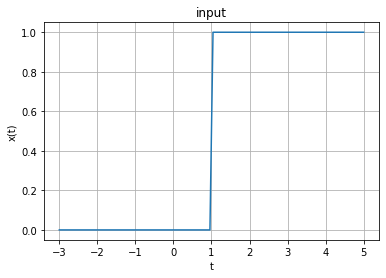
\includegraphics[width=\columnwidth]{GateAssignment1(1).png}
 \caption{Plot of $x(t)$}
 \label{plot}
\end{figure}

\begin{figure}[!h]
 \centering
 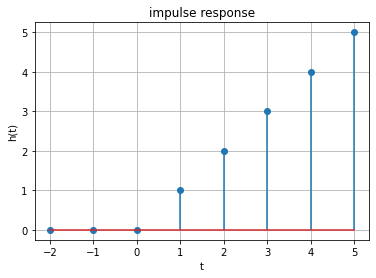
\includegraphics[width=\columnwidth]{GateAssignment1(2).png}
 \caption{Plot of $h(t)$}
 \label{plot}
\end{figure}

\begin{figure}[!h]
 \centering
 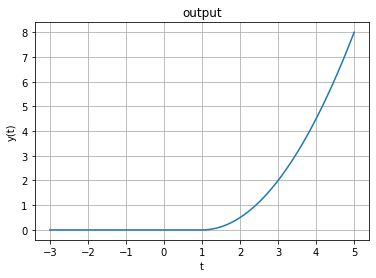
\includegraphics[width=\columnwidth]{GateAssignment1(3).png}
 \caption{Plot of $y(t)$}
 \label{plot}
\end{figure}
\end{document}


